% !TeX spellcheck = da_DK
\subsection{Forstærker i tilpasningsblok}
\subsubsection{Teori og design}
Jævnfør i afsnit \ref{Subsec:Forstaerker} på side \pageref{Subsec:Forstaerker} er der forklaret teorien samt designet af en forstærker, hvilket også gør sig gældende her. Da denne blok skal tilpasse det filtrerede signal til komparatoren, afgrænses måleintervallet til $\pm25^{\circ}$. Et range på $\pm90^{\circ}$ er unødvendigt ift. at vurdere hvorvidt patienten er faldet. Derfor ønskes det, at $V_{out}$ fra denne forstærker er $\pm3$V, når accelerometret måler $\pm25^{\circ}$. Denne forstærkning skal derved forstærke med en faktor 3, hvilket svarer til $9.5424$dB, som beskrevet i afsnit \ref{Tilpasningsblok} på side \pageref{Tilpasningsblok}. \\
For at udregne modstandene er R$2$ blevet valgt til $10$K$\Omega$. Ud fra dette er R$1$ blevet bestemt ved følgende udregning:
\begin{align}
3 = 1 + (\frac{R1}{10\text{K}\Omega})\\
R1 = 20\text{K}\Omega
\end{align}

\noindent Forstærkerens opbygning kan ses på \figref{fig:Forstaerker_faktor3}.
\begin{figure}[H]
	\centering
	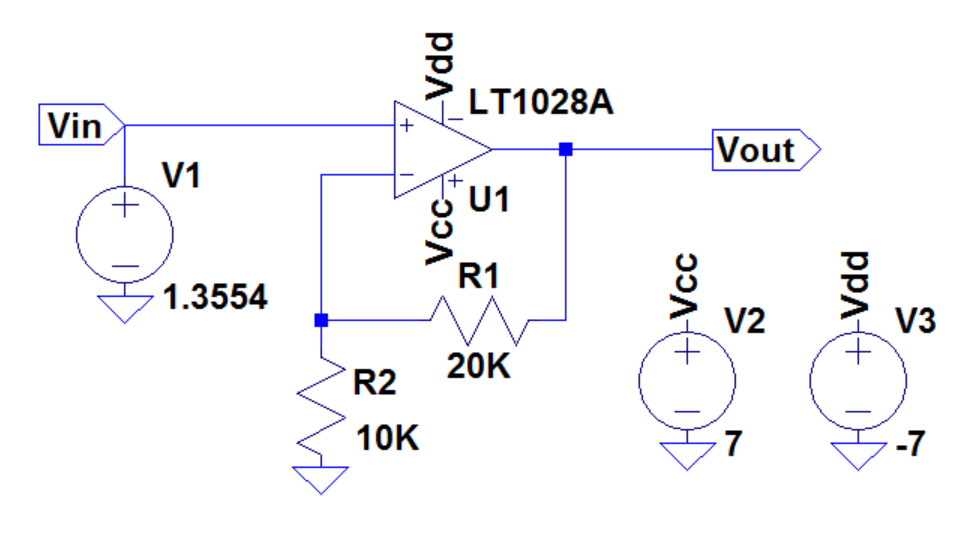
\includegraphics[scale=0.4]{figures/cProblemloesning/Forstaerker_faktor3.PNG}
	\caption{På figuren ses den ikke-inverterende opbygningen af forstærkeren, hvor der sker en forstærkning med en faktor $3$.}
	\label{fig:Forstaerker_faktor3}
\end{figure}

\subsubsection{Simulering}
Denne forstærker undersøges i fire simuleringer for, hvorledes forstærkeren virker. Det forstærkede signal, kaldet $V_{out}$, skal være $3$ gange større end $V_{in}$. Resultaterne af fire simuleringer ses i \tableref{tab:forstarker3_simT}. Der er benyttet de teoretiske værdier, som er udregnet fra start.
\begin{table}[H]
	\centering
	\begin{tabular}{|l|l|l|l|l|l|}
		\hline
		\multicolumn{1}{|c|}{\textit{Inputsignalet}} & \multicolumn{1}{c|}{\textit{Forstærkning}} & \multicolumn{1}{c|}{\textit{Forventet outputsignal}}                      & \multicolumn{1}{c|}{\textit{Outputsignalet}} & \textit{Forstærkning}  & \multicolumn{1}{c|}{\textit{Afvigelse}} \\ \hline
		$2.7096$V     & 3   & \begin{tabular}[c]{@{}l@{}}Forventer mætning\\ $8.1288$V\end{tabular}  & $3.9765$V  & $\times$ & $\times$     \\ \hline
		$0.8325$V     & 3   & $2.4975$V                                                              & $2.4975$V  & $3$ & $0\%$     \\ \hline
%		$0$V          & 3   & $0$V                                                                   & $33.6527\mu $V        & $\approx 0\%$     \\ \hline
	   -$0.8100$V     & 3   & -$2.4300$V                                                             & -$2.4299$V  & $3$ & $0.004\%$     \\ \hline
	   -$2.6388$V     & 3   & \begin{tabular}[c]{@{}l@{}}Forventer mætning\\ -$7.9164$V\end{tabular} & -$3.9770$V  & $\times$ & $\times$     \\ \hline
	\end{tabular}
		\caption{I tabellen ses resultaterne af de fire simuleringer.}
		\label{tab:forstarker3_simT}
\end{table}
Der ses i \tableref{tab:forstarker3_simT} , at der ingen afvigelse er i forstærkningen. Kredsløbet fungere rent teoretisk med ideelle komponenter, som bliver brugt i LTspice. På \figref{fig:faktor3_simulering} ses simuleringen af $0.8325$V input, som ideelt vil komme fra filtret, hvis accelerometret hælder i $25^{\circ}$.

\begin{figure}[H]
	\centering
	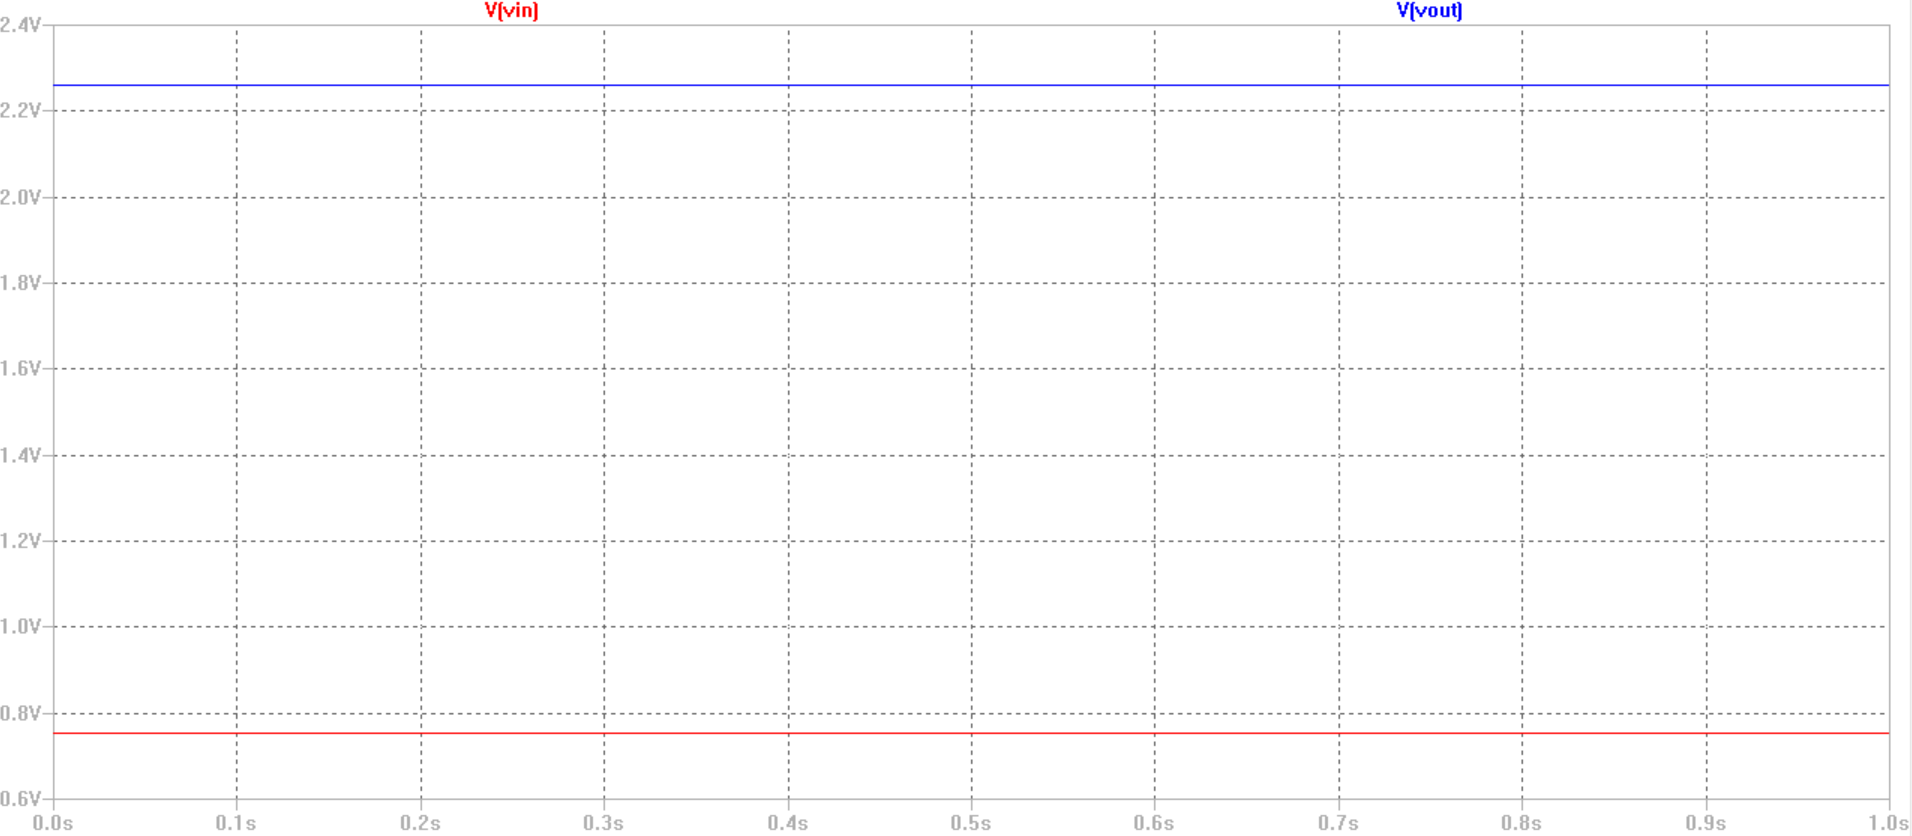
\includegraphics[scale=0.4]{figures/cProblemloesning/Forstaerker_faktor3_simulering.PNG}
	\caption{På figuren ses simuleringen af $0.8325$V input, som giver $2.4975$V i output. Der er altså sket en forstærkning med en faktor $3$.}
	\label{fig:faktor3_simulering}
\end{figure}
\noindent Der ses på afvigelserne, at der arbejdes med ideelle komponenter. Det er herved bevist, at kredsløbet fungerer teoretisk og kan derfor implementeres.

\subsubsection{Implementering og test}
På \figref{fig:Forstaerker_faktor3} kan der ses, at der skal benyttes to modstandere på $10$K$\Omega$ og $20$K$\Omega$ til opbygningen af forstærkeren med en faktor på 3. Reelt findes der dog ikke en $20$K$\Omega$, hvorfor der istedet benyttes to $10$K$\Omega$ modstandere i serieforbindelse, hvilket teoretisk vil give en $0$\% afvigelse fra en ideelt $20$K$\Omega$ modstander. Disse tre modstandere blev målt inden testen, hvilket fremgår i \tableref{Tab:modstand_faktor18}.
\begin{table}[H]
	\centering
	\begin{tabular}{|l|l|l|}
		\hline
		\textit{Teoretisk}  & \textit{Ved måling} & \textit{\% afvigelse} \\ \hline
		$10$K$\Omega$       & $99.8$K$\Omega$     & $0.2$\%               \\ \hline
		$10$K$\Omega$       & $99.8$K$\Omega$     & $0.2$\%               \\ \hline
		$10$K$\Omega$       & $10$K$\Omega$       & $0$\%               \\ \hline
	\end{tabular}
	\caption{I tabellen ses der, at de tre modstandere afviger lidt fra deres teoretiske værdi, hvilket er forventet af reelle komponenter. Det er dog en acceptabel afvigelse, så modstanderne kan derfor anvendes til implementeringen.}
	\label{Tab:modstand_faktor18}
\end{table}

\noindent Herefter implementeres kredsløbet. Til opsamling af signalet benyttes en computer med ScopeLogger, hvorefter dataen bliver behandlet i Matlab. I testen blev der foretaget tre målinger for hver af de fire spændingsniveauer. Herefter blev gennemsnittet for hver måling udregnet, som lægges sammen og til slut også tages gennemsnittet af. Dette giver den endelige værdi, som står under "Output" i \tableref{Tab:faktor3_test}.\

\begin{table}[H]
	\centering
	\begin{tabular}{|l|l|l|l|l|}
		\hline
 \textit{Input} & \textit{Forventet output} & \textit{Output}  &  \textit{Forstærkning}  & \% afvigelse \\ \hline
 $2.7096$V            & Mætning              & $4.8210$V       &    $\times$             & $\times$  \\ \hline
 $0.8325$V            & $2.2623$V            & $2.2569$V       &    $2.99$               & $0.33\%$     \\ \hline
%		$0$V                   & $-1.030$mV           & $-3.090$mV                & $-6.200$mV      &              \\ \hline
-$0.8100$V           & $2.2158$V            & -$2.2247$V       &    $3.01$               & $0.33\%$     \\ \hline
-$2.6388$V           & Mætning              & -$4.1536$V       &    $\times$             & $\times$    \\ \hline
	\end{tabular}
	\caption{I tabellen ses resultaterne fra testen med forstærkeren, der har en faktor 3.}
	\label{Tab:faktor3_test}
\end{table}

For $2.7096$, $0.8325$V og -$0.8100$ er spændingen kommet direkte fra en strømforsyning, men for at undersøge forstærkningen af -$2.6388$V er det nødsaget at benytte offsettet samt faktor 9 forstærkeren, da spændingsforsyningen ikke kan levere en så stor negativ spænding. Det var derfor forventet, at der kunne være en større afvigelse på målingerne med -$2.6388$V spænding, da denne spænding skulle igennem flere kredsløb. Inputtet i offsettet (som kan ses på \figref{fig:Offset_generisk}) udregnes på følgende måde:
\begin{equation}\label{Udregnxfaktor3}
( x - 1.5902V ) * 9 = -XXX \\
x =
\end{equation}
Reference blev målt til $XX$V og via teorien vides det, at den ønskede spænding skulle være -$2.6388$V. I \eqref{Udregnxfaktor3} udregnes inputspændingen til offsettet til at være $XX$V. Denne blev sat til $XX$V, som gav et output på $-0.2640$V, der blev sendt ind i faktor 9 forstærkeren. Herefter var outputtet i gennemsnit -$XX$V, som blev sendt ind i faktor 3 forstærkeren. Dette gav i gennemsnit outputtet $XX$V, som ses i \tableref{Tab:faktor3_test}. %Afvigelsen, som ville opstå grundet to ekstra kredsløb ift. de to andre målinger, ville være præsentabel for afvigelsen, som der også burde have været for de to andre spændingers tests. 
Der ses i \tableref{Tab:faktor3_test}, at der ikke opstod større forstyrrelser trods flere sammensatte systemer, der ville give ekstra afvigelse i det målte signal ift. det forventede signal. \\
Der ses ud fra testen, at forstærkeren overholder kravene fra afsnit \ref{OpsamlingsAfs} på side \pageref{OpsamlingsAfs} samt ligger inde for tolerancerne.